\documentclass[pdf]{beamer}
\ProvidesPackage{preamble_slides}

% %% Beamer Stuff
\usetheme{Berlin}
\setbeamertemplate{footline}[frame number]
\setbeamertemplate{caption}[numbered]
\setbeamertemplate{section in toc}[sections numbered]
\setbeamertemplate{subsection in toc}[sections numbered]
\setbeamertemplate{navigation symbols}{} 
\setbeamercovered{transparent=25}
\usepackage{graphicx}
\usepackage{hhline}
\usepackage{appendixnumberbeamer}
\usepackage{multirow}
\definecolor{maincolor}{rgb}{0.6, 0.4, 0.7}
\usecolortheme[named = maincolor]{structure}
\renewcommand{\arraystretch}{1.5}

%% Bibliography packages
\usepackage{natbib}
\bibliographystyle{abbrvnat}

\title{Chinese Head Tax Project: Updates}
\author{Amy Kim}
\date{August 8, 2023}

\begin{document}
\begin{frame}[plain]
    \titlepage
\end{frame}

\begin{frame}{Research Question}
    How does an increase in fixed migration costs (in the form of a nationality-specific flat `head tax' at the time of entry) affect selection into immigration?
\end{frame}

% PART 1: IMMIGRATION INFLOW EFFECTS
\section{Immigration Inflow}
\begin{frame}[label = data1]
    \frametitle{Data Issues}
    \textbf{Ferenczi and Willcox (1929)}
    \begin{itemize}
        \item Immigration by country and year only starts in 1900 (no pre-period data for Head Tax)
        \item Census data is mostly similar in shape, but differs significantly at times \hyperlink{flow_compar_all}{\beamerbutton{All Countries}} \hyperlink{flow_compar_belgium}{\beamerbutton{Belgium}}  \hyperlink{flow_compar_japan}{\beamerbutton{Japan}}
    \end{itemize}
    \textbf{Time Series Emigration Regressions à la Hatton and Williamson (1994)}
    \begin{itemize}
        \item Essentially missing any origin country data for China (wages, population, industrialization)
        \item Don't have annual Chinese population in Canada -- okay to impute between decennial censuses?
    \end{itemize}
\end{frame}

\begin{frame}[label = flow_reg]
    \frametitle{Immigration Inflow: Regression Specification}
    \begin{multline}
        \text{FLOW}_t = \alpha + \beta_1\text{TOTALIMM}_t + \beta_2\text{GNPGROWTH}_t +  \\ \delta_1 t + \delta_2 t^2 + \sum_{\tau \in \mathcal{T}} \gamma_\tau \mathbf{1}[TAX_t = \tau] 
    \end{multline}
    \begin{itemize}
        \item Same as regression from last time, 1880-1910 to cut out WWI
    \end{itemize}
\end{frame}

\begin{frame}[label = country_regs]
    \frametitle{Graphing $\gamma_\tau$'s for Various Countries [Eq (1)]}
    \begin{figure}
        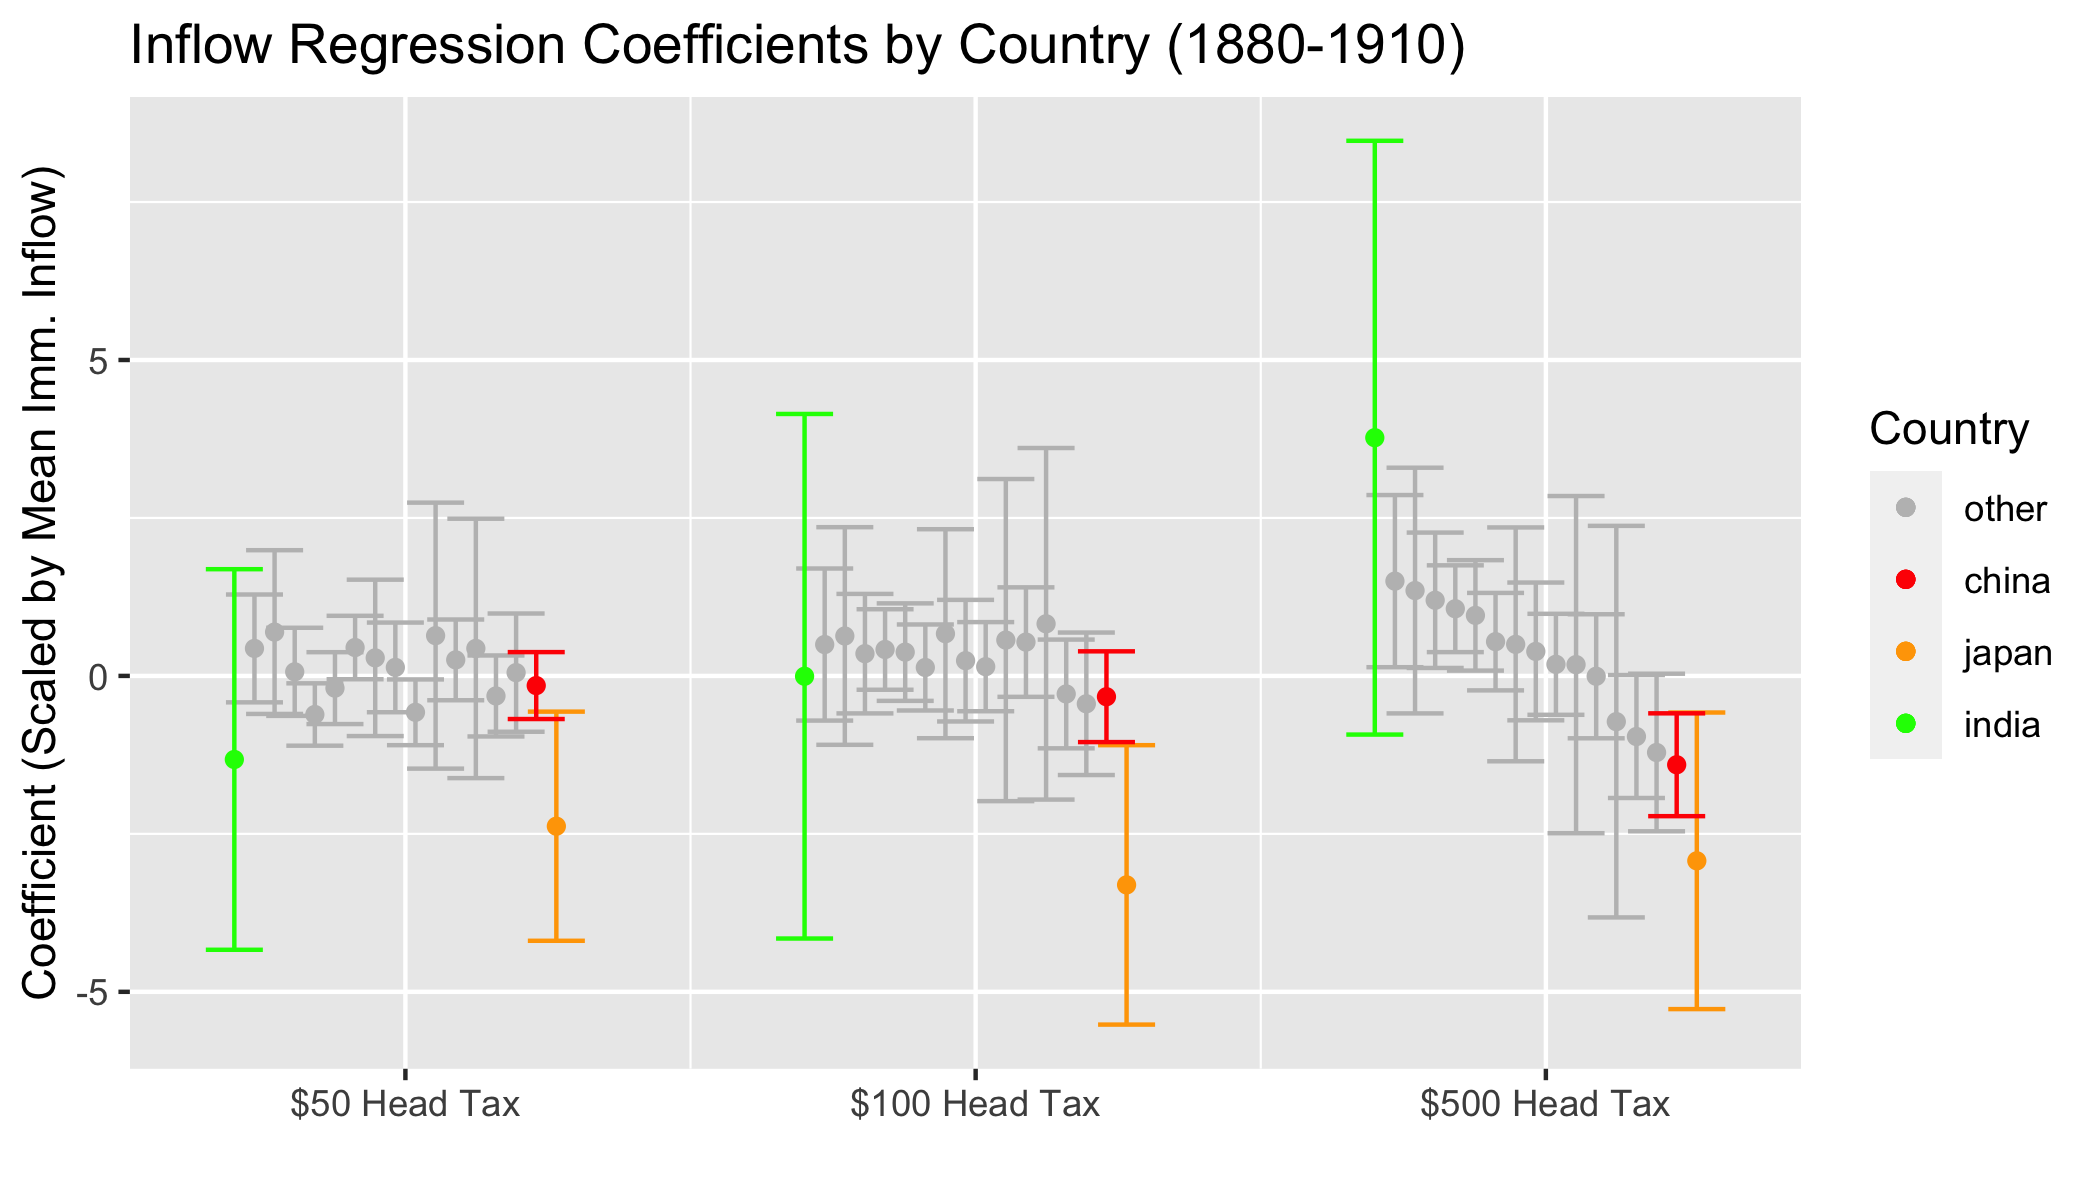
\includegraphics[width = \textwidth]{../../figs/8aug23/reg_coefs.png}
    \end{figure}
    \scriptsize
    Countries (L to R): India, Belgium, Australia/NZ, France, Poland, Russia, Italy, Denmark, Norway, Germany, Switzerland, Sweden, West Indies, Austria/Hungary, Finland, China, Japan
\end{frame}

\begin{frame}[label = tab2_flow]
    \frametitle{Immigration Inflow: Sig. Effects on Japanese Immigration?}
    \centering
    \begin{table}[H]
		\resizebox{\textwidth}{!}{
            
% Table created by stargazer v.5.2.3 by Marek Hlavac, Social Policy Institute. E-mail: marek.hlavac at gmail.com
% Date and time: Mon, Jul 17, 2023 - 15:10:09
\begin{tabular}{@{\extracolsep{5pt}}lccccc} 
\\[-1.8ex]\hline 
\hline \\[-1.8ex] 
 & \multicolumn{5}{c}{\textit{Dependent variable:}} \\ 
\cline{2-6} 
\\[-1.8ex] & $CHIFLOW^R$ (Register) & $CHIFLOW^C$ (Census) & $JAPANFLOW^C$ (Census) & $CHIFLOW^C$ (Pre-1908) & $JAPANFLOW^C$ (Pre-1908) \\ 
\\[-1.8ex] & (1) & (2) & (3) & (4) & (5)\\ 
\hline \\[-1.8ex] 
 \$50 Tax &  & $-$453.700 & $-$383.200 & $-$96.840 & $-$56.450 \\ 
  &  & (399.800) & (242.300) & (294.200) & (187.600) \\ 
  & & & & & \\ 
 \$100 Tax & $-$695.100 & $-$599.000 & $-$867.000$^{**}$ & $-$283.200 & $-$1,089.000$^{***}$ \\ 
  & (834.500) & (604.800) & (366.500) & (353.100) & (225.100) \\ 
  & & & & & \\ 
 \$500 Tax & $-$6,989.000$^{***}$ & $-$1,607.000$^{**}$ & $-$810.100$^{*}$ & $-$1,188.000$^{**}$ & $-$1,620.000$^{***}$ \\ 
  & (1,006.000) & (669.300) & (405.600) & (471.200) & (300.500) \\ 
  & & & & & \\ 
\hline \\[-1.8ex] 
Observations & 38 & 41 & 41 & 28 & 28 \\ 
Adjusted R$^{2}$ & 0.747 & 0.675 & 0.430 & 0.730 & 0.833 \\ 
\hline 
\hline \\[-1.8ex] 
\textit{Note:}  & \multicolumn{5}{r}{$^{*}$p$<$0.1; $^{**}$p$<$0.05; $^{***}$p$<$0.01} \\ 
\end{tabular} 

		}
	\end{table}  
    \hyperlink{census_flow}{\beamerbutton{Census Inflow w/ Japanese Imm.}}
\end{frame}

% % PART 2: IMMIGRANT COMPOSITION EFFECTS
% \section{Immigrant Composition}
% \begin{frame}[label = tab3_old_spec]
%     \frametitle{Immigrant Composition: Initial Specification}
%     \centering
%     \begin{itemize}
%         \item \textbf{Full Sample Info:} 4-5\% samples from 1901, 1911, 1921 censuses which include year of arrival to Canada
%         \item \textbf{Initial Specification:} for arrival year $t$, only keep observations from closest census year (e.g. only keep 1901 census observations for 1900 arrivals; only keep 1911 census observations for 1901 \& 1902 arrivals, etc.)
%         \begin{equation*}
%             y_{it} = \delta_t + \alpha CHI_i + \sum_{\tau \in \{100,500\}} \gamma_{\tau} CHI_i \times \mathbf{1}[TAX_t = \tau] + \varepsilon_{it}
%         \end{equation*}
%         \item $\delta_t$ absorbs both arrival year and census year fixed effects 
%         \item No controls for age (but just age ctrl doesn't change much)
%         \item Limit sample to adult men; arrival year 1890 and after
%     \end{itemize}
%     \hyperlink{tab3_old}{\beamerbutton{Results}}
% \end{frame}

% \begin{frame}[label = tab3_new_spec1]
%     \frametitle{Immigrant Composition: Modifications}
%     \centering
%     \begin{itemize}
%         \item Col (1) is original regression for labor [(4) Japanese Only]
%         \item Col (2) expands sample to all years of arrival [(5) Japanese Only]
%         \item \textbf{New Specification:} col (3) [(6) Japanese Only] keeps all census year $c$ x arrival year $t$ observations (e.g. for 1900 arrivals, have observations from 1901, 1911, and 1921 censuses)
%         \begin{equation*}
%             y_{itc} = \beta_c + \delta_t + \alpha CHI_i + \sum_{\tau \in \{100,500\}} \gamma_{\tau} CHI_i \times \mathbf{1}[TAX_t = \tau] + \varepsilon_{it}
%         \end{equation*}
%         \item Now $\beta_c$ absorbs census year FE separately from arrival year FE $\delta_t$ 
%         \item Col (3) also controls for age \textbf{and} age at arrival [(6) Japanese Only]
%     \end{itemize}
% \end{frame}

% \begin{frame}[label = tab3_new_labor]
% 	\frametitle{Outcome Regressions: LABORER}
%     \centering
%     \begin{table}[H]
% 		\resizebox{\textwidth}{!}{
%             
% Table created by stargazer v.5.2.3 by Marek Hlavac, Social Policy Institute. E-mail: marek.hlavac at gmail.com
% Date and time: Thu, Jul 20, 2023 - 16:52:44
\begin{tabular}{@{\extracolsep{5pt}}lcccccc} 
\\[-1.8ex]\hline 
\hline \\[-1.8ex] 
 & All (1890-1920) & All (1870-1920) & All (All Census Yrs) & Japan. (1890-1908) & Japan. (1870-1908) & Japan. (All Census Yrs) \\ 
\\[-1.8ex] & (1) & (2) & (3) & (4) & (5) & (6)\\ 
\hline \\[-1.8ex] 
 $BORNCHI$ & 0.146$^{***}$ & 0.128$^{***}$ & 0.201$^{***}$ & $-$0.026 & 0.042 & $-$0.039 \\ 
  & (0.022) & (0.035) & (0.024) & (0.041) & (0.270) & (0.209) \\ 
  & & & & & & \\ 
 $BORNCHI \times$ \$50 Tax &  & 0.019 & $-$0.035 &  & $-$0.063 & 0.077 \\ 
  &  & (0.040) & (0.027) &  & (0.273) & (0.211) \\ 
  & & & & & & \\ 
 $BORNCHI \times$ \$100 Tax & 0.050 & 0.068 & 0.032 & 0.005 & $-$0.063 & 0.110 \\ 
  & (0.037) & (0.046) & (0.031) & (0.088) & (0.281) & (0.218) \\ 
  & & & & & & \\ 
 $BORNCHI \times$ \$500 Tax & $-$0.050$^{**}$ & $-$0.031 & $-$0.100$^{***}$ & $-$0.106$^{*}$ & $-$0.174 & $-$0.038 \\ 
  & (0.025) & (0.037) & (0.026) & (0.064) & (0.275) & (0.213) \\ 
  & & & & & & \\ 
\hline \\[-1.8ex] 
Observations & 42,058 & 47,802 & 85,139 & 1,383 & 1,619 & 3,121 \\ 
Adjusted R$^{2}$ & 0.025 & 0.029 & 0.052 & 0.006 & 0.008 & 0.016 \\ 
\hline \\[-1.8ex] 
\end{tabular} 

% 		}
% 	\end{table}  
% \end{frame}

% \begin{frame}[label = tab3_new_canread]
% 	\frametitle{Outcome Regressions: CANREAD}
%     \centering
%     \begin{table}[H]
% 		\resizebox{\textwidth}{!}{
%             
% Table created by stargazer v.5.2.3 by Marek Hlavac, Social Policy Institute. E-mail: marek.hlavac at gmail.com
% Date and time: Thu, Jul 20, 2023 - 16:52:44
\begin{tabular}{@{\extracolsep{5pt}}lcccccc} 
\\[-1.8ex]\hline 
\hline \\[-1.8ex] 
 & All (1890-1920) & All (1870-1920) & All (All Census Yrs) & Japan. (1890-1908) & Japan. (1870-1908) & Japan. (All Census Yrs) \\ 
\\[-1.8ex] & (1) & (2) & (3) & (4) & (5) & (6)\\ 
\hline \\[-1.8ex] 
 $BORNCHI$ & $-$0.305$^{***}$ & $-$0.313$^{***}$ & $-$0.344$^{***}$ & $-$0.147$^{***}$ & $-$0.445$^{*}$ & $-$0.292 \\ 
  & (0.018) & (0.027) & (0.018) & (0.052) & (0.266) & (0.208) \\ 
  & & & & & & \\ 
 $BORNCHI \times$ \$50 Tax &  & 0.016 & 0.128$^{***}$ &  & 0.323 & 0.308 \\ 
  &  & (0.032) & (0.020) &  & (0.271) & (0.210) \\ 
  & & & & & & \\ 
 $BORNCHI \times$ \$100 Tax & 0.146$^{***}$ & 0.154$^{***}$ & 0.134$^{***}$ & 0.384$^{***}$ & 0.682$^{**}$ & 0.365$^{*}$ \\ 
  & (0.026) & (0.033) & (0.022) & (0.095) & (0.278) & (0.217) \\ 
  & & & & & & \\ 
 $BORNCHI \times$ \$500 Tax & 0.030 & 0.037 & 0.081$^{***}$ & 0.076 & 0.374 & 0.201 \\ 
  & (0.020) & (0.029) & (0.019) & (0.072) & (0.271) & (0.211) \\ 
  & & & & & & \\ 
\hline \\[-1.8ex] 
Observations & 41,212 & 46,767 & 83,910 & 1,051 & 1,201 & 2,657 \\ 
Adjusted R$^{2}$ & 0.043 & 0.047 & 0.053 & 0.026 & 0.033 & 0.014 \\ 
\hline \\[-1.8ex] 
\end{tabular} 

% 		}
% 	\end{table}  
% \end{frame}

% \begin{frame}[label = tab3_new_earn]
% 	\frametitle{Outcome Regressions: EARN}
%     \centering
%     \begin{table}[H]
% 		\resizebox{\textwidth}{!}{
%             
% Table created by stargazer v.5.2.3 by Marek Hlavac, Social Policy Institute. E-mail: marek.hlavac at gmail.com
% Date and time: Thu, Jul 20, 2023 - 16:52:45
\begin{tabular}{@{\extracolsep{5pt}}lcccccc} 
\\[-1.8ex]\hline 
\hline \\[-1.8ex] 
 & All (1890-1920) & All (1870-1920) & All (All Census Yrs) & Japan. (1890-1908) & Japan. (1870-1908) & Japan. (All Census Yrs) \\ 
\\[-1.8ex] & (1) & (2) & (3) & (4) & (5) & (6)\\ 
\hline \\[-1.8ex] 
 $BORNCHI$ & $-$250.800$^{***}$ & $-$263.800$^{***}$ & $-$509.200$^{***}$ & $-$29.790$^{**}$ & $-$76.010 & $-$151.000 \\ 
  & (37.760) & (63.520) & (96.770) & (12.760) & (82.580) & (130.500) \\ 
  & & & & & & \\ 
 $BORNCHI \times$ \$50 Tax &  & 11.080 & 150.100 &  & 48.140 & 106.000 \\ 
  &  & (71.880) & (107.800) &  & (83.580) & (131.900) \\ 
  & & & & & & \\ 
 $BORNCHI \times$ \$100 Tax & $-$59.340 & $-$46.260 & 59.300 & 78.100$^{***}$ & 124.300 & $-$53.420 \\ 
  & (65.340) & (81.980) & (124.500) & (27.520) & (86.370) & (137.400) \\ 
  & & & & & & \\ 
 $BORNCHI \times$ \$500 Tax & $-$152.100$^{***}$ & $-$139.000$^{**}$ & 70.950 & 47.490$^{**}$ & 93.700 & 28.800 \\ 
  & (43.710) & (67.030) & (104.100) & (20.770) & (84.310) & (133.100) \\ 
  & & & & & & \\ 
\hline \\[-1.8ex] 
Observations & 27,635 & 30,981 & 51,461 & 1,125 & 1,296 & 2,381 \\ 
Adjusted R$^{2}$ & 0.121 & 0.128 & 0.047 & 0.293 & 0.260 & 0.231 \\ 
\hline \\[-1.8ex] 
\end{tabular} 

% 		}
% 	\end{table}  
% \end{frame}

% \begin{frame}[label = tab3_new_houseown]
% 	\frametitle{Outcome Regressions: HOUSEOWN}
%     \centering
%     \begin{table}[H]
% 		\resizebox{\textwidth}{!}{
%             
% Table created by stargazer v.5.2.3 by Marek Hlavac, Social Policy Institute. E-mail: marek.hlavac at gmail.com
% Date and time: Thu, Jul 20, 2023 - 16:52:45
\begin{tabular}{@{\extracolsep{5pt}}lcccccc} 
\\[-1.8ex]\hline 
\hline \\[-1.8ex] 
 & All (1890-1920) & All (1870-1920) & All (All Census Yrs) & Japan. (1890-1908) & Japan. (1870-1908) & Japan. (All Census Yrs) \\ 
\\[-1.8ex] & (1) & (2) & (3) & (4) & (5) & (6)\\ 
\hline \\[-1.8ex] 
 $BORNCHI$ & $-$0.260$^{***}$ & $-$0.405$^{***}$ & $-$0.469$^{***}$ & 0.024 & $-$0.048 & $-$0.131 \\ 
  & (0.024) & (0.039) & (0.028) & (0.031) & (0.217) & (0.171) \\ 
  & & & & & & \\ 
 $BORNCHI \times$ \$50 Tax &  & 0.135$^{***}$ & 0.114$^{***}$ &  & 0.063 & 0.009 \\ 
  &  & (0.045) & (0.031) &  & (0.220) & (0.172) \\ 
  & & & & & & \\ 
 $BORNCHI \times$ \$100 Tax & $-$0.156$^{***}$ & $-$0.012 & 0.079$^{**}$ & $-$0.240$^{***}$ & $-$0.168 & $-$0.017 \\ 
  & (0.041) & (0.051) & (0.036) & (0.068) & (0.226) & (0.177) \\ 
  & & & & & & \\ 
 $BORNCHI \times$ \$500 Tax & $-$0.053$^{*}$ & 0.092$^{**}$ & 0.182$^{***}$ & $-$0.099$^{**}$ & $-$0.027 & 0.013 \\ 
  & (0.028) & (0.042) & (0.030) & (0.049) & (0.221) & (0.173) \\ 
  & & & & & & \\ 
\hline \\[-1.8ex] 
Observations & 42,058 & 47,802 & 85,139 & 1,383 & 1,619 & 3,121 \\ 
Adjusted R$^{2}$ & 0.078 & 0.103 & 0.170 & 0.039 & 0.041 & 0.051 \\ 
\hline \\[-1.8ex] 
\end{tabular} 

% 		}
% 	\end{table}  
% \end{frame}

% \begin{frame}
%     \frametitle{Outcome Regressions: Key Takeaways}
%     \centering
%     \begin{itemize}
%         \item Not sure if Japanese are good comparison group (very small sample, also had some immigration restrictions)
%         \item Changing the year of arrival span (col 2) doesn't change much for all immigrant sample -- likely because pre-1890 Chinese immigrant pop is relatively small anyways
%         \item For all immigrant comparison sample -- mostly results are the same (suggestive of some positive selection on literacy/likelihood of being a laborer) although there is no longer evidence of effects on earnings 
%         \item $BORNCHI \times$ \$500 Tax coefficient for HOUSEOWN flips with new specification -- now \textbf{positive}, suggesting positive selection outweighs wealth effects of the tax 
%     \end{itemize}
% \end{frame}

% \begin{frame}
%     \frametitle{Next Steps}
%     \centering
%     \begin{itemize}
%         \item Figuring out correct comparison group (matched sample?)
%         \item Finalizing regression specifications
%         \item Visualization of outcome regressions -- maybe plotting DiD coeffs?
%         \item Repeating for US data 
%     \end{itemize}
% \end{frame}
%%%%%%%%%%%%%%%%%%%%%%%%%%%%%%%%%%%%%%%%%%%%%%%%%%%%%%%
%%%%%%%%%%      A  P  P  E  N  D  I  X      %%%%%%%%%%%
%%%%%%%%%%%%%%%%%%%%%%%%%%%%%%%%%%%%%%%%%%%%%%%%%%%%%%%
\appendix

%---------------------------
%  Census/NBER Immflow Comparisons
%---------------------------
\begin{frame}[label = flow_compar_all]
	\frametitle{NBER vs. Census Immigration Data}
    \centering
	\begin{figure}[H]
		\begin{center}
			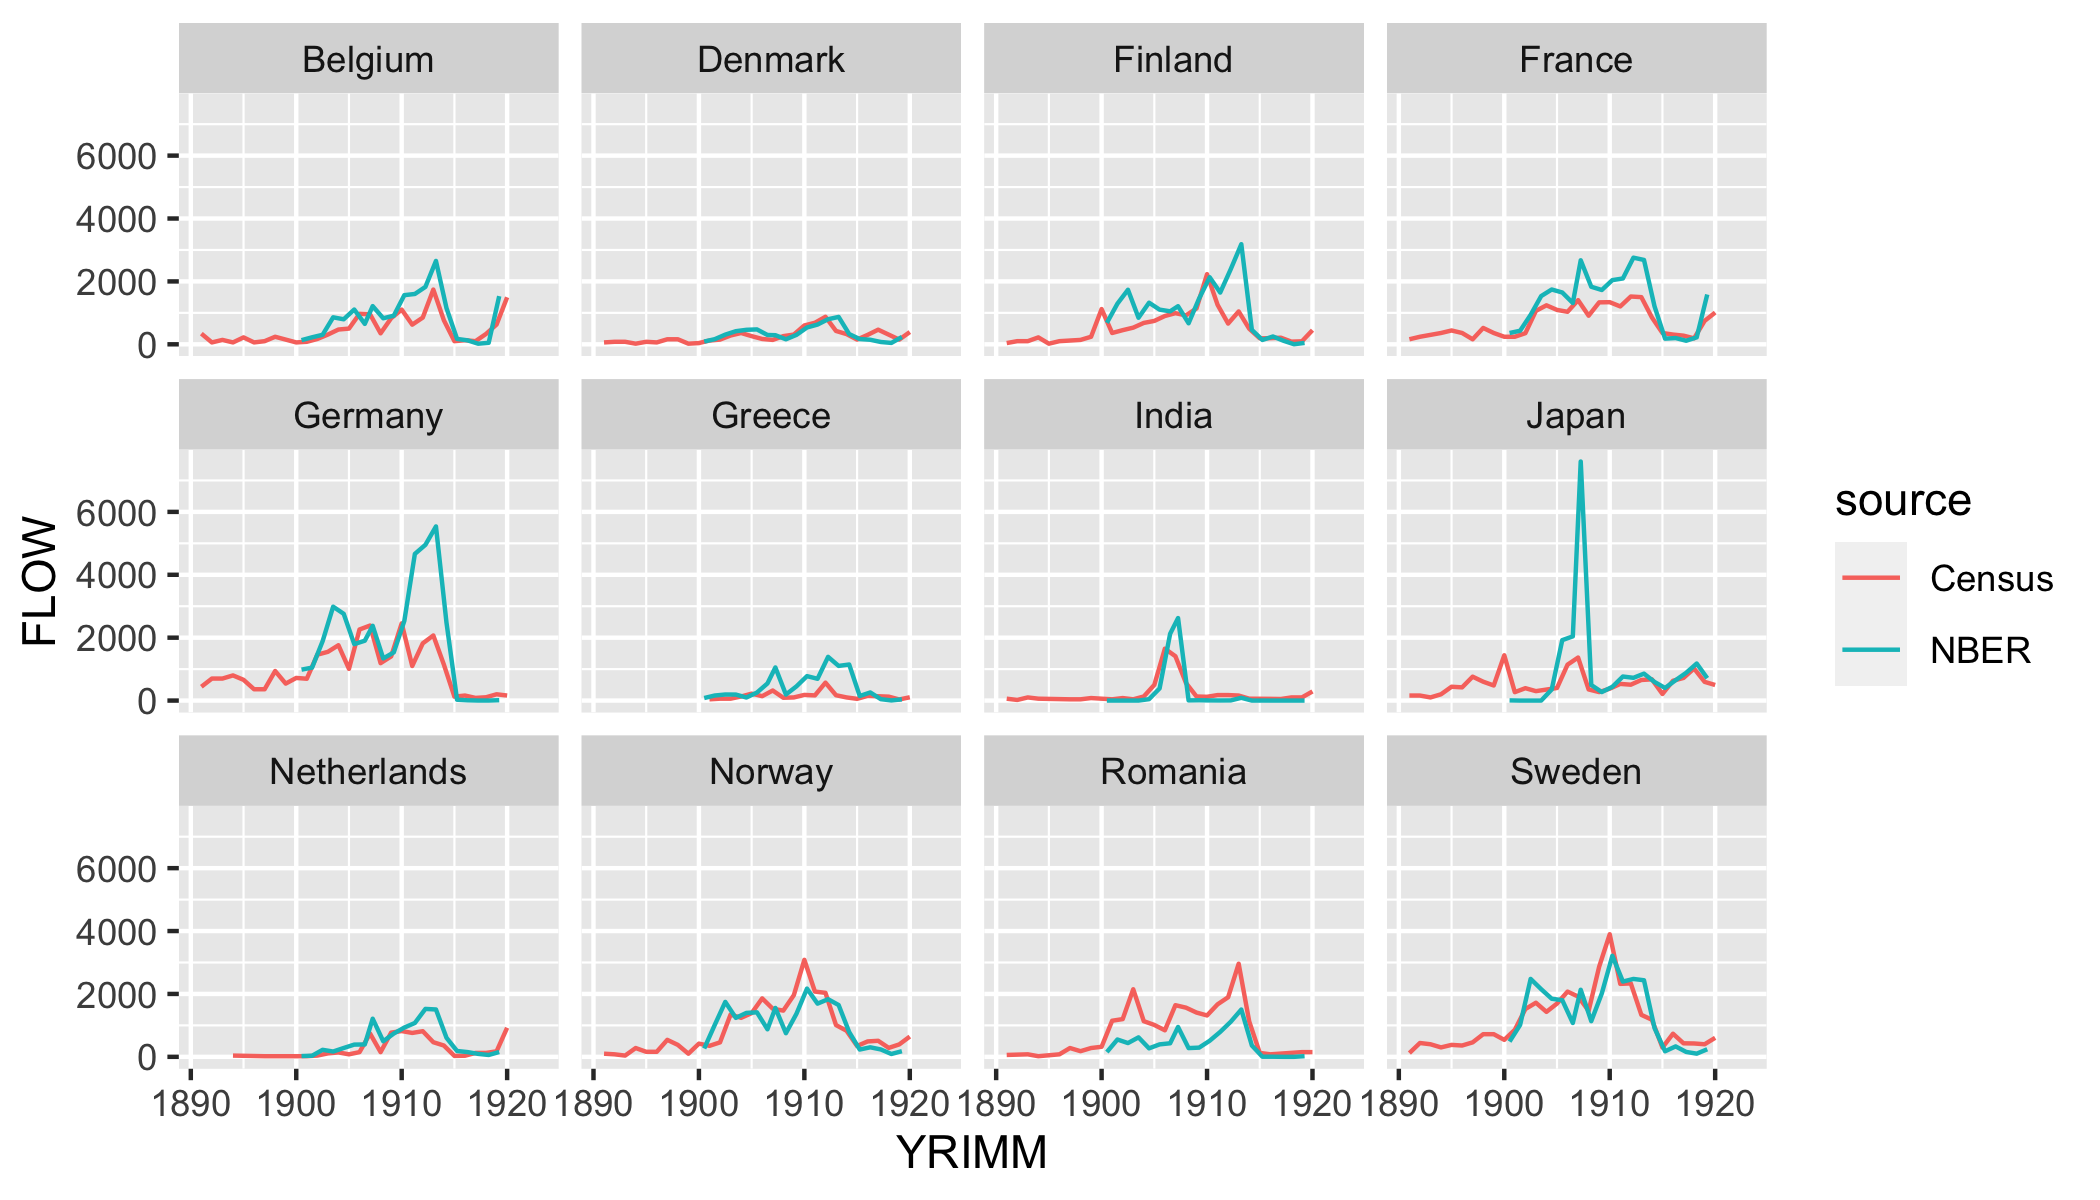
\includegraphics[width=\textwidth]{../../figs/8aug23/nber_census_compare_all.png}
		\end{center}
	\end{figure}
    \hyperlink{data1}{\beamerbutton{Back to Slides}}
\end{frame}

\begin{frame}[label = flow_compar_belgium]
	\frametitle{NBER vs. Census Immigration Data: Belgium}
    \centering
	\begin{figure}[H]
		\begin{center}
			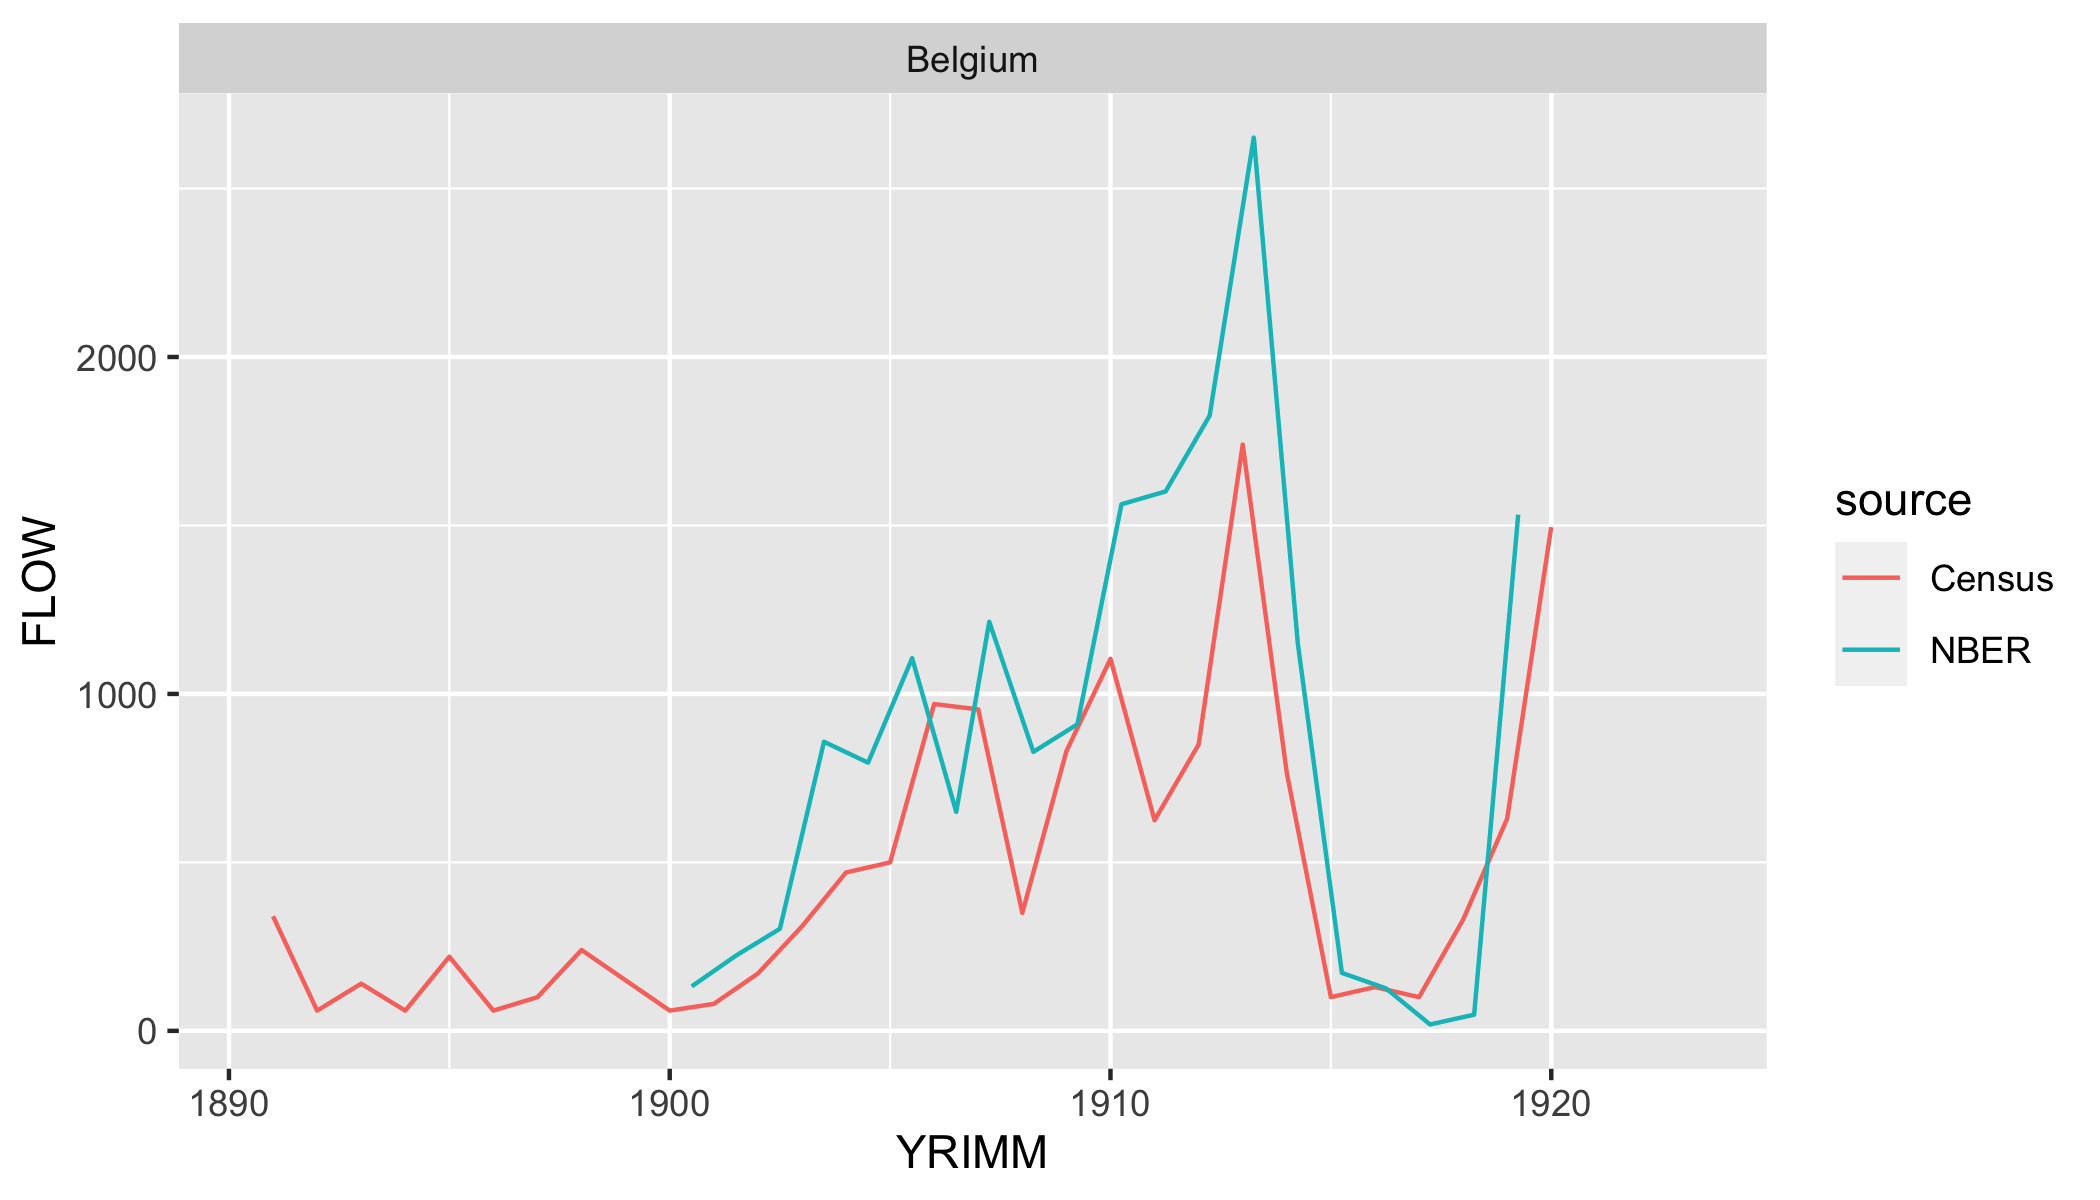
\includegraphics[width=\textwidth]{../../figs/8aug23/nber_census_compare_belgium.png}
		\end{center}
	\end{figure}
    \hyperlink{data1}{\beamerbutton{Back to Slides}}
\end{frame}


\begin{frame}[label = flow_compar_japan]
	\frametitle{NBER vs. Census Immigration Data: Japan}
    \centering
	\begin{figure}[H]
		\begin{center}
			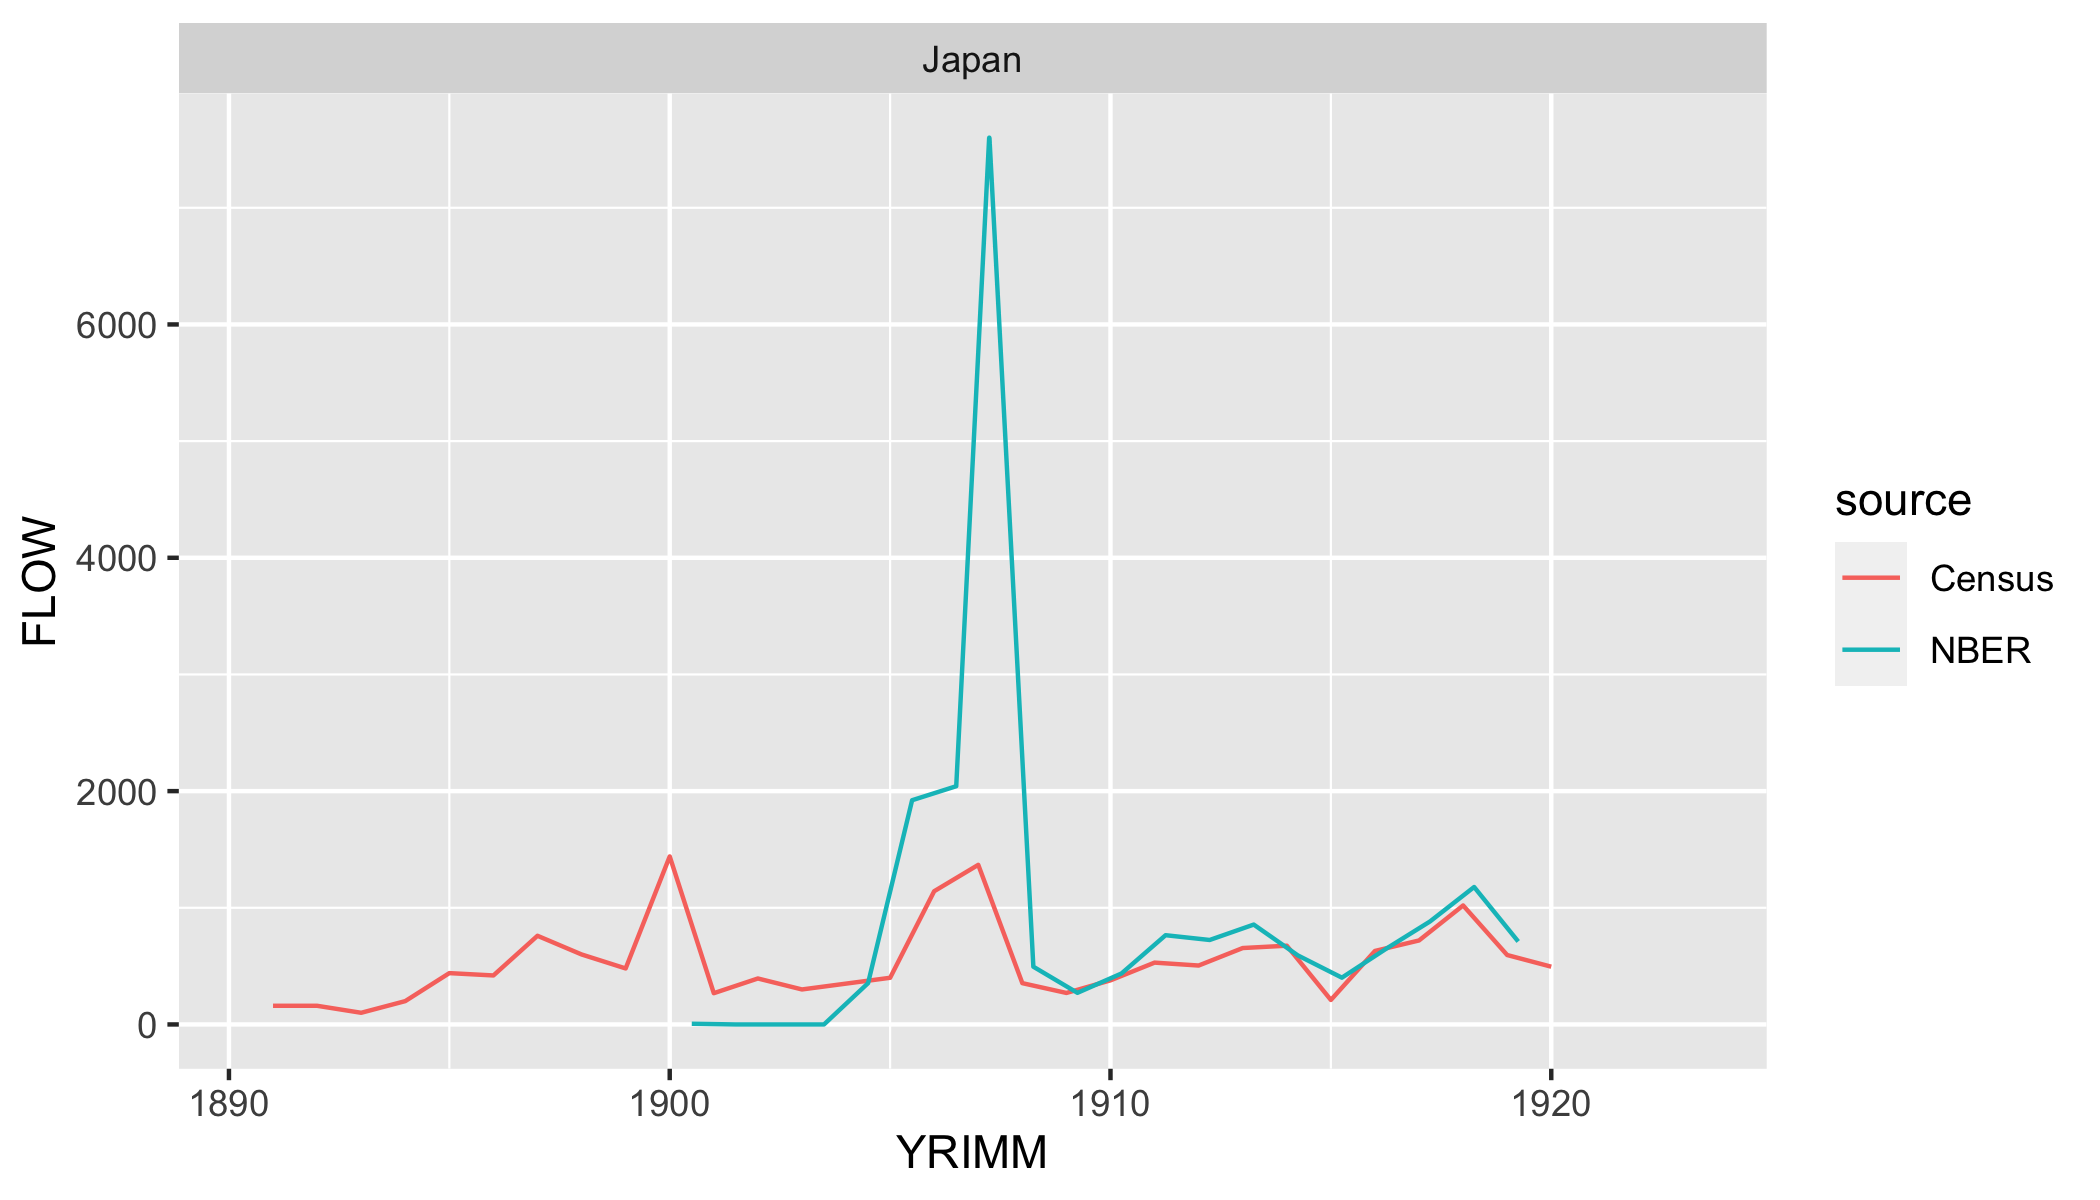
\includegraphics[width=\textwidth]{../../figs/8aug23/nber_census_compare_japan.png}
		\end{center}
	\end{figure}
    \hyperlink{data1}{\beamerbutton{Back to Slides}}
\end{frame}

% %---------------------------
% %  Normalized Chinese Inflow (Inflow Diff)
% %---------------------------

% \begin{frame}[label = flow_diff]
% 	\frametitle{Chinese Immigration Inflow as Fraction of Total}
%     \centering
% 	\begin{figure}[H]
% 		\begin{center}
% 			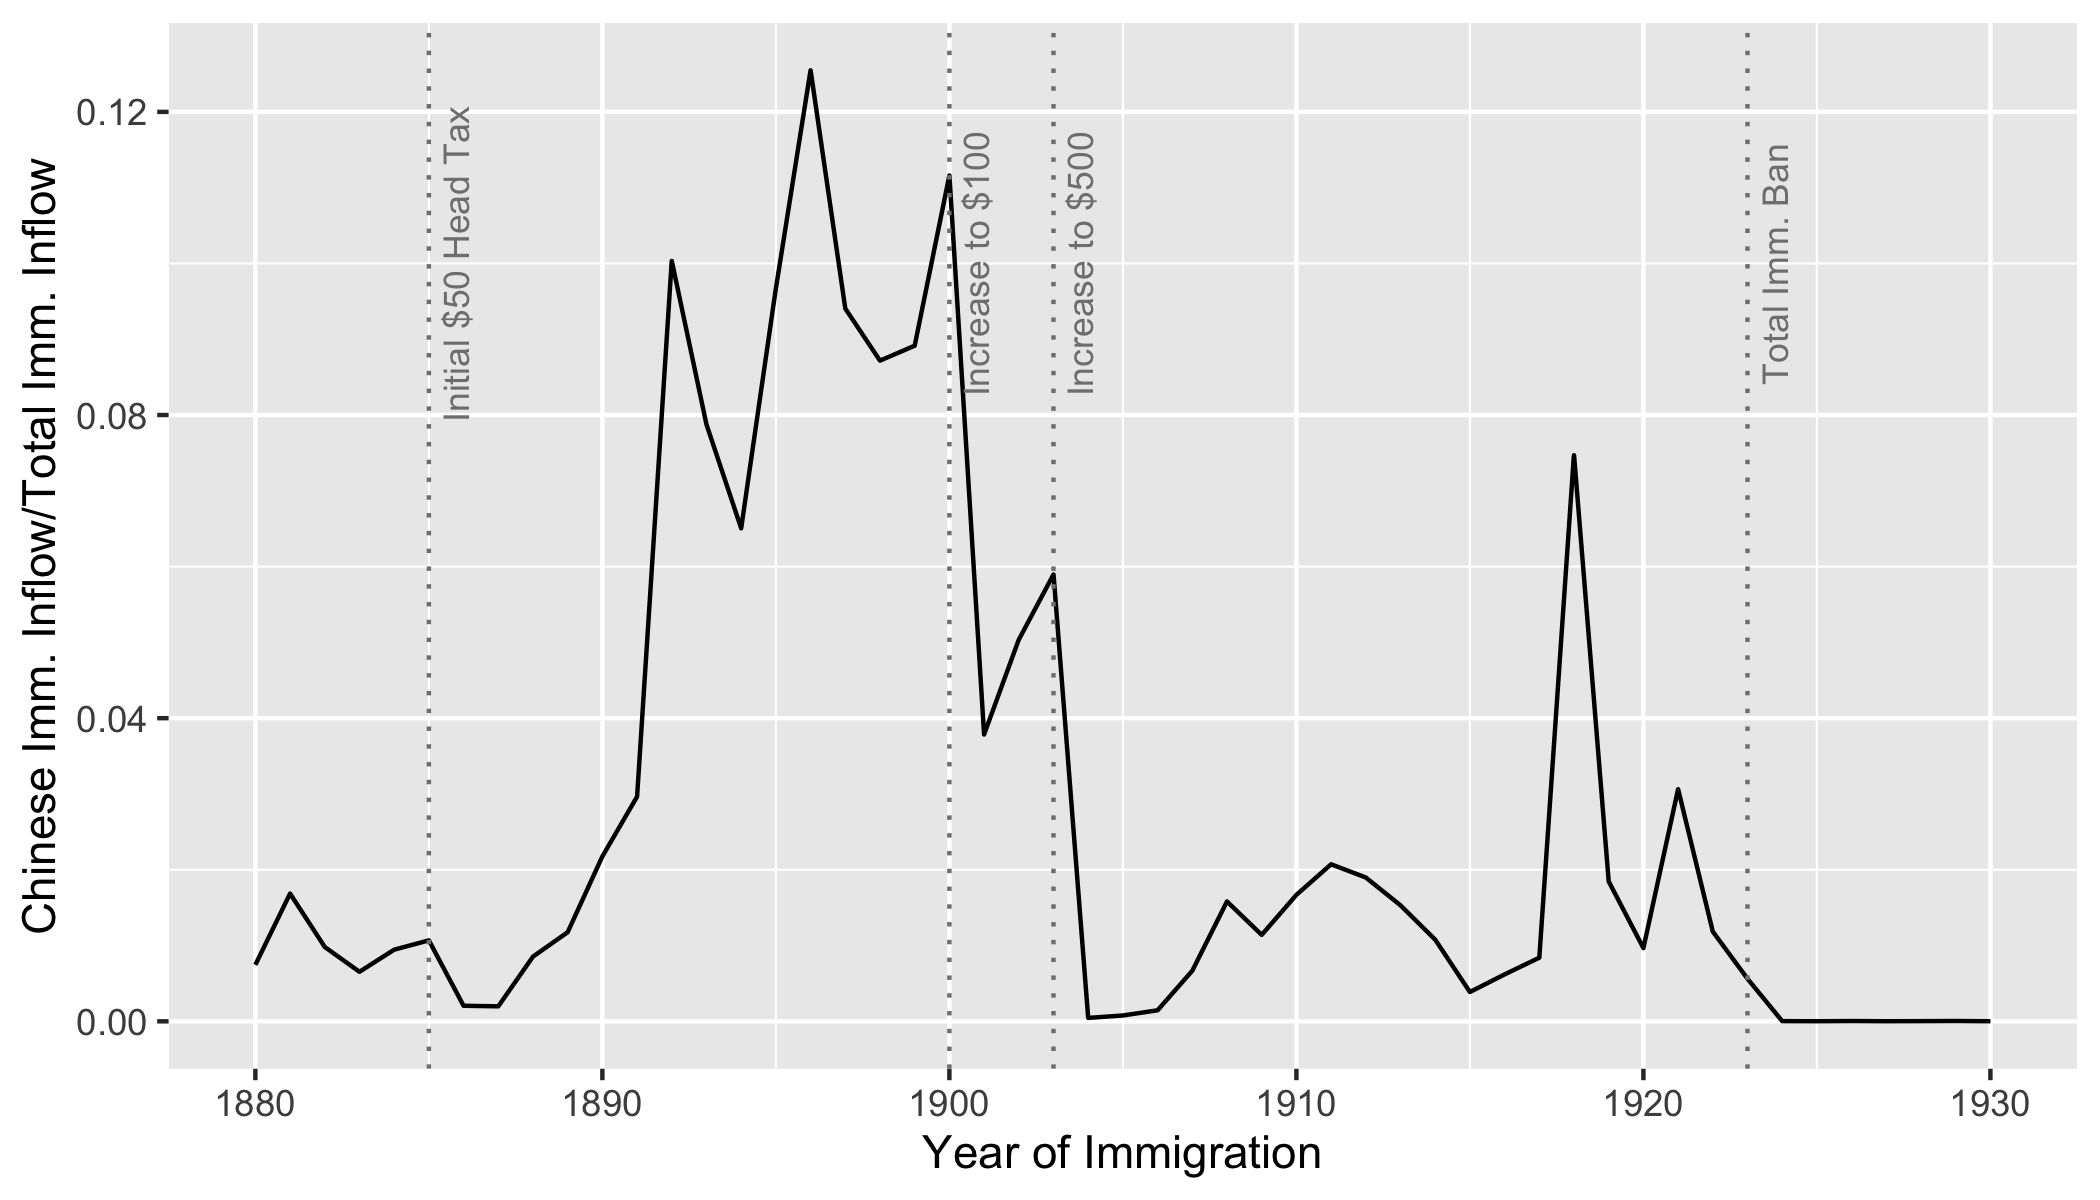
\includegraphics[width=\textwidth]{../../figs/21jul23/flowpct.png}
% 		\end{center}
% 	\end{figure}
%     \hyperlink{flow_reg}{\beamerbutton{Back to Slides}}
% \end{frame}

% %---------------------------
% %  Census Inflow w/ Japanese
% %---------------------------

% \begin{frame}[label = census_flow]
% 	\frametitle{Immigration Inflow with Census Data}
%     \centering
% 	\begin{figure}[H]
% 		\begin{center}
% 			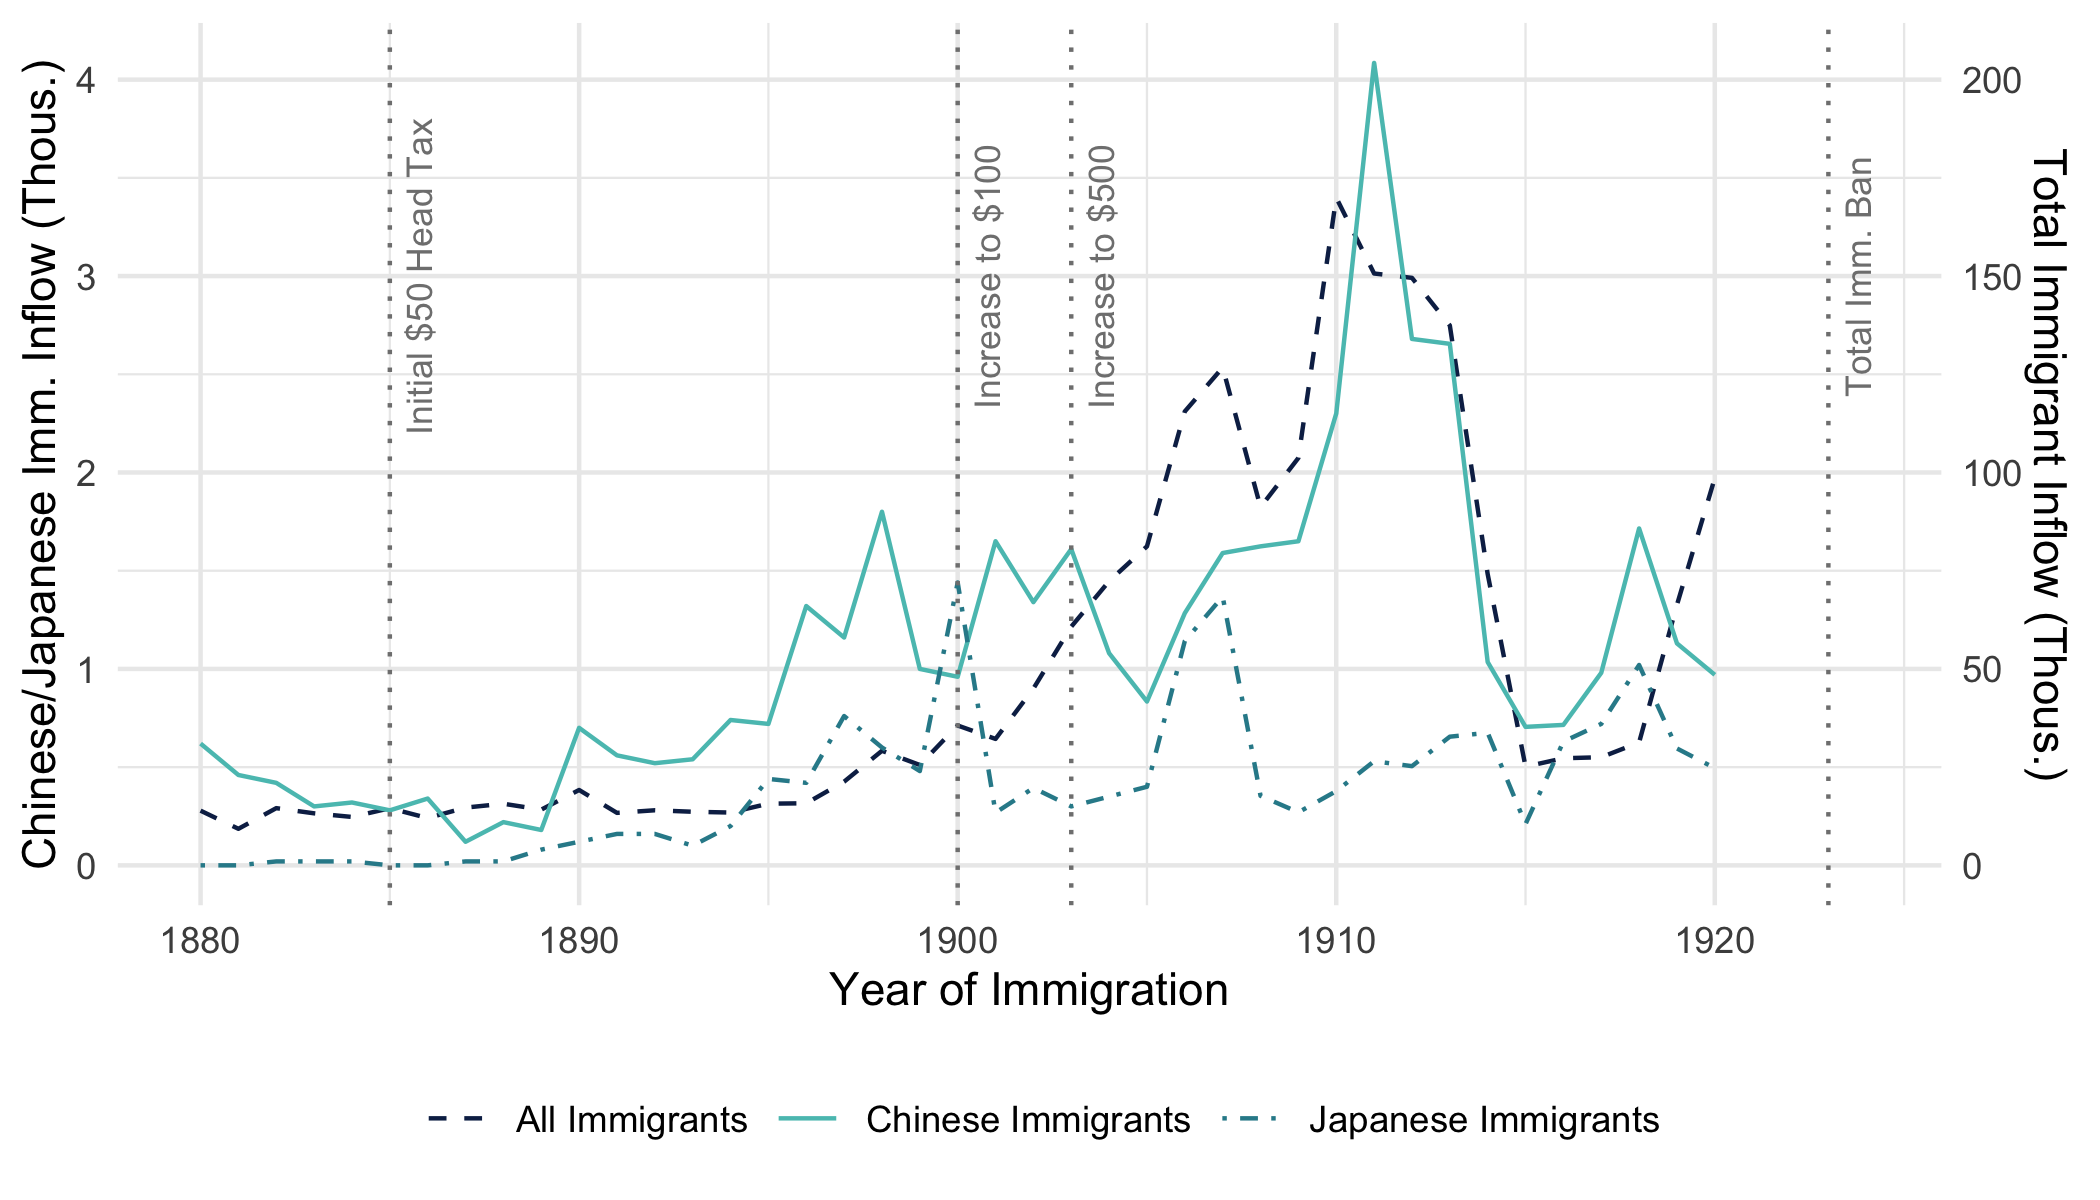
\includegraphics[width=\textwidth]{../../figs/21jul23/fig2_flow_jap.png}
% 		\end{center}
% 	\end{figure}
%     \hyperlink{tab2_flow}{\beamerbutton{Back to Slides}}
% \end{frame}


% %---------------------------
% %  Old outcome regs (all imm. only)
% %---------------------------

% \begin{frame}[label = tab3_old]
% 	\frametitle{Outcome Regressions w/ Old Specification}
%     \centering
%     \begin{table}[H]
% 		\resizebox{\textwidth}{!}{
%             
% Table created by stargazer v.5.2.3 by Marek Hlavac, Social Policy Institute. E-mail: marek.hlavac at gmail.com
% Date and time: Wed, Jul 19, 2023 - 22:56:43
\begin{tabular}{@{\extracolsep{5pt}}lcccccccc} 
\\[-1.8ex]\hline 
\hline \\[-1.8ex] 
 & \multicolumn{4}{c}{All Immigrants (1890-1920)} & \multicolumn{4}{c}{Chinese/Japanese Immigrants (1890-1908)} \\ 
 & \multicolumn{8}{c}{\textit{Dependent variable:}} \\ 
\cline{2-9} 
\\[-1.8ex] & $LABORER$ & $LITERATE$ & $EARNINGS$ & $HOMEOWN$ & $LABORER$ & $LITERATE$ & $EARNINGS$ & $HOMEOWN$ \\ 
\\[-1.8ex] & (1) & (2) & (3) & (4) & (5) & (6) & (7) & (8)\\ 
\hline \\[-1.8ex] 
 $BORNCHI$ & 0.146$^{***}$ & $-$0.305$^{***}$ & $-$250.800$^{***}$ & $-$0.260$^{***}$ & $-$0.026 & $-$0.147$^{***}$ & $-$29.790$^{**}$ & 0.024 \\ 
  & (0.022) & (0.018) & (37.760) & (0.024) & (0.041) & (0.052) & (12.760) & (0.031) \\ 
  & & & & & & & & \\ 
 $BORNCHI \times$ \$100 Tax & 0.050 & 0.146$^{***}$ & $-$59.340 & $-$0.156$^{***}$ & 0.005 & 0.384$^{***}$ & 78.100$^{***}$ & $-$0.240$^{***}$ \\ 
  & (0.037) & (0.026) & (65.340) & (0.041) & (0.088) & (0.095) & (27.520) & (0.068) \\ 
  & & & & & & & & \\ 
 $BORNCHI \times$ \$500 Tax & $-$0.050$^{**}$ & 0.030 & $-$152.100$^{***}$ & $-$0.053$^{*}$ & $-$0.106$^{*}$ & 0.076 & 47.490$^{**}$ & $-$0.099$^{**}$ \\ 
  & (0.025) & (0.020) & (43.710) & (0.028) & (0.064) & (0.072) & (20.770) & (0.049) \\ 
  & & & & & & & & \\ 
Includes Year FE & Yes & Yes & Yes & Yes & Yes & Yes & Yes & Yes \\ 
\hline \\[-1.8ex] 
Observations & 42,058 & 41,212 & 27,635 & 42,058 & 1,383 & 1,051 & 1,125 & 1,383 \\ 
Adjusted R$^{2}$ & 0.025 & 0.043 & 0.121 & 0.078 & 0.006 & 0.026 & 0.293 & 0.039 \\ 
\hline \\[-1.8ex] 
\end{tabular} 

% 		}
% 	\end{table}  
%     \hyperlink{tab3_old_spec}{\beamerbutton{Back to Slides}}
% \end{frame}


\end{document}